\documentclass{article}


% Language setting
% Replace `english' with e.g. `spanish' to change the document language
\usepackage[english]{babel}

% Set page size and margins
% Replace `letterpaper' with `a4paper' for UK/EU standard size
\usepackage[letterpaper,top=2cm,bottom=2cm,left=3cm,right=3cm,marginparwidth=1.75cm]{geometry}

% Useful packages
\usepackage{amsmath,amsthm}
\usepackage{graphicx}
\usepackage[colorlinks=true, allcolors=blue]{hyperref}


\newtheorem{remark}{Remark}



\title{WeatherGenerator Architecture}
\author{Christian Lessig \\ {\small European Centre for Medium-Range Weather Forecasts, Bonn, Germany} \\ {\small \href{mailto:christian.lessig@ecmwf.int}{christian.lessig@ecmwf.int}}}

\begin{document}
\maketitle


\begin{figure}[h!]
	\centering
	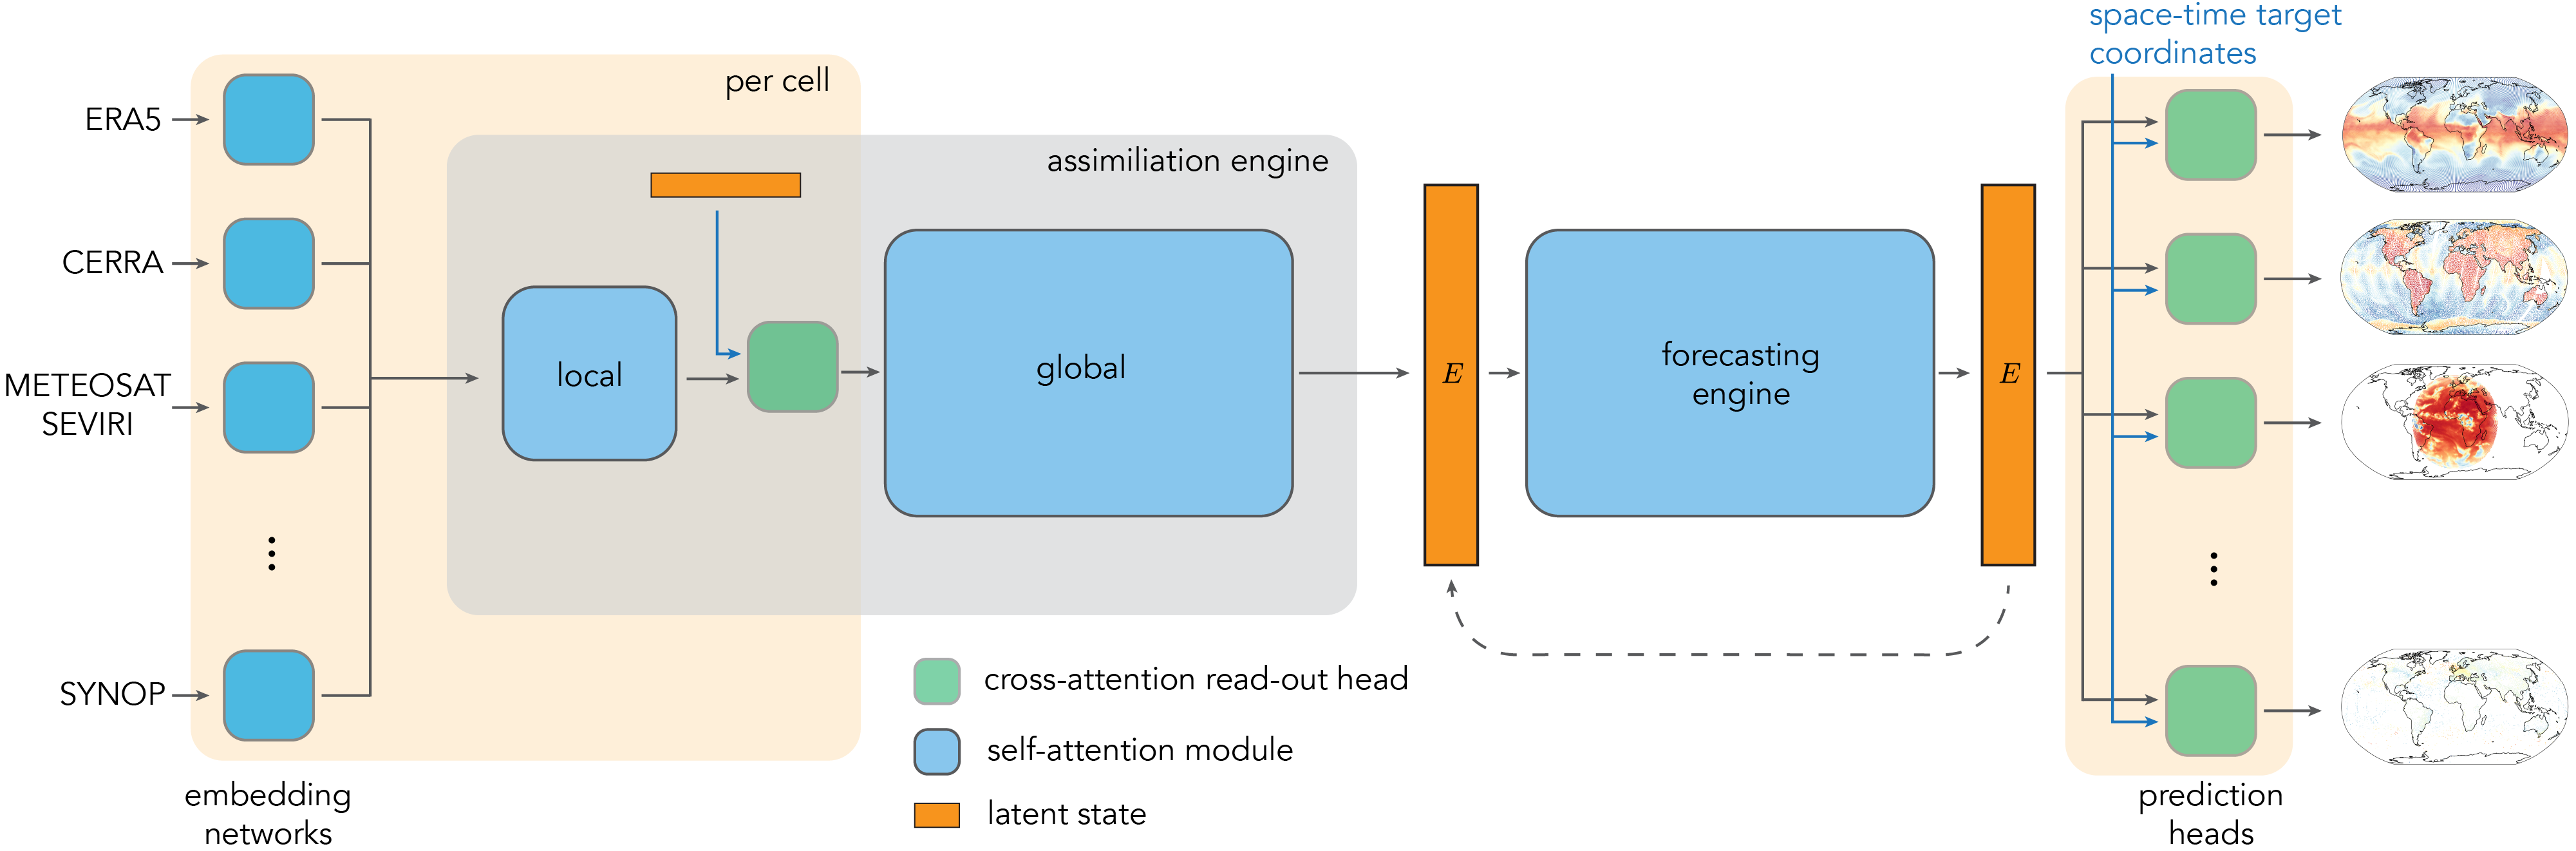
\includegraphics[width=\textwidth]{figures/arch.png}
    % 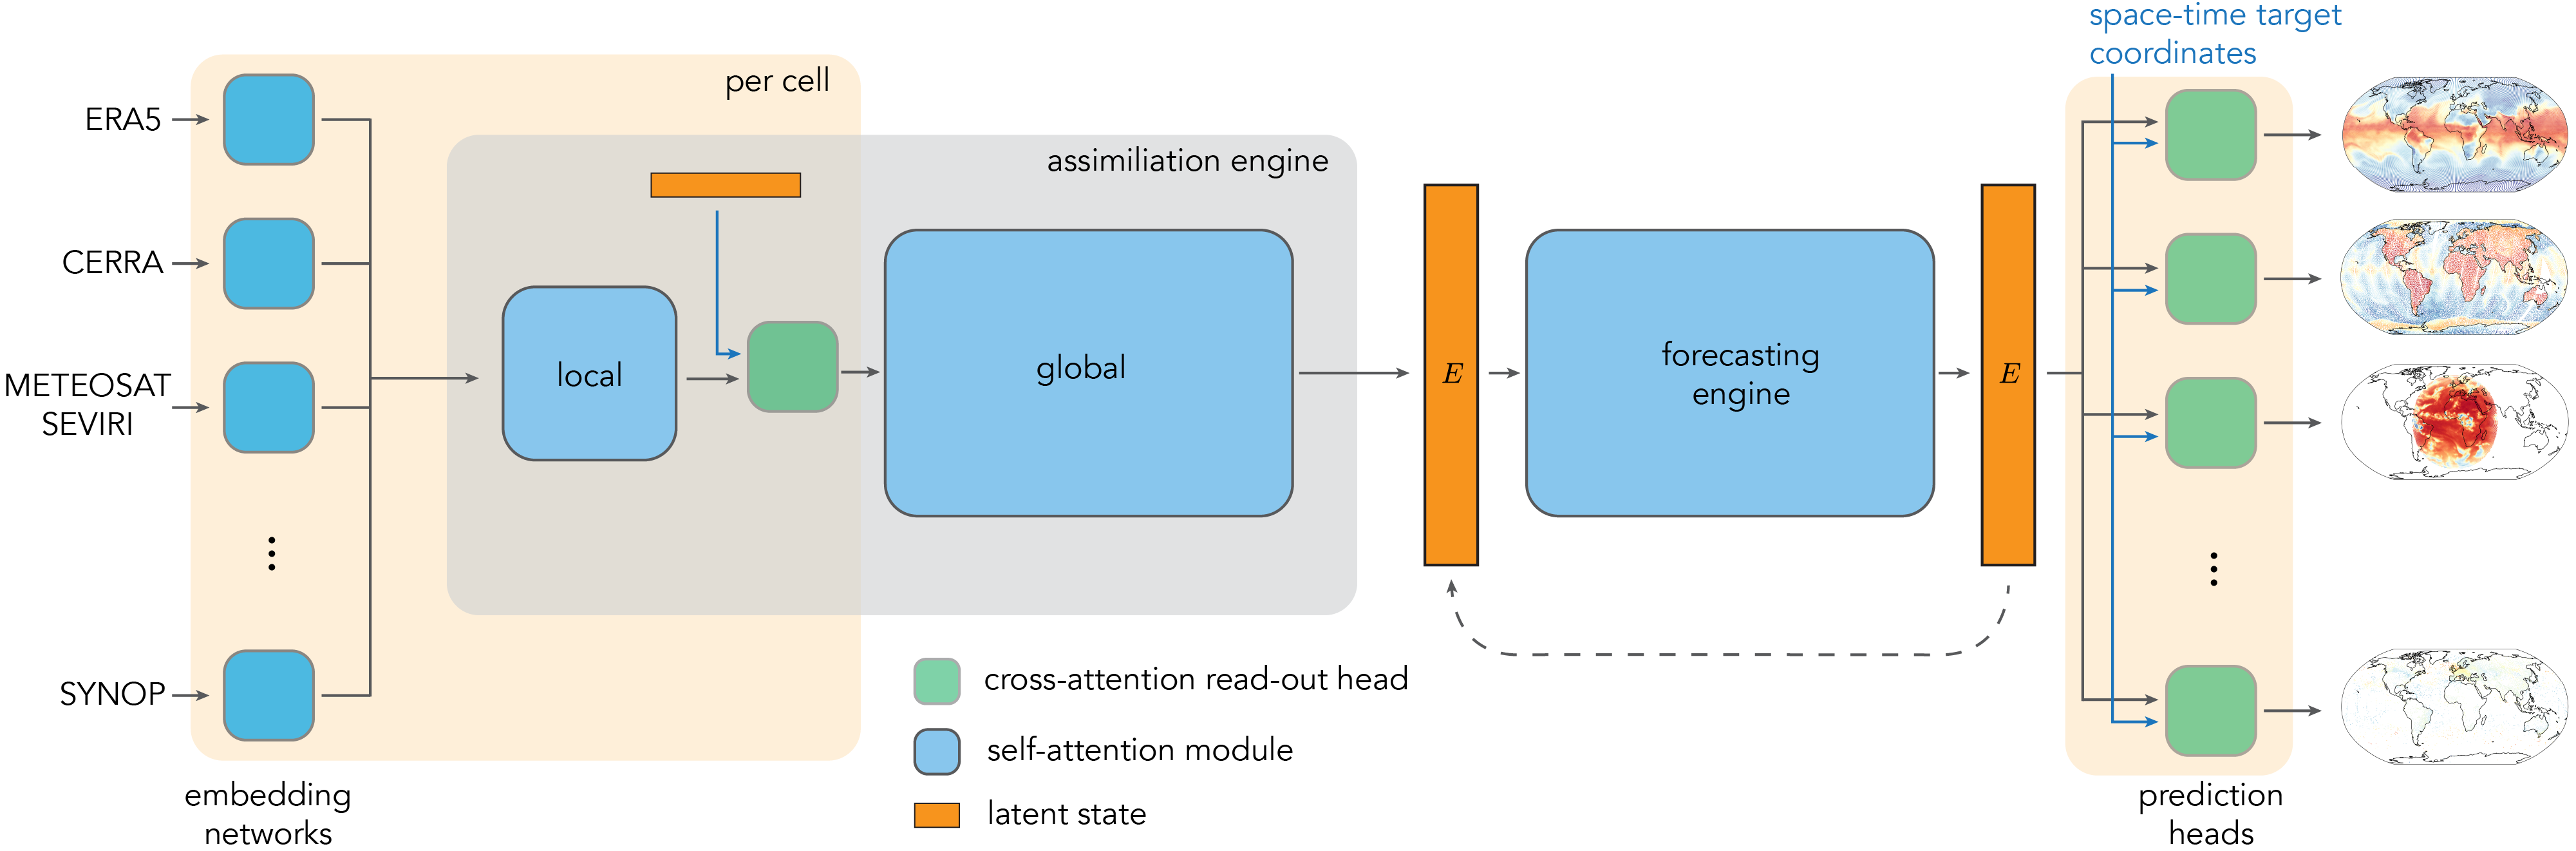
\includegraphics[width=\textwidth]{figures/arch.pdf}
	\caption{Overview of the WeatherGenerator neural network architecture}
	\label{fig:arch}
\end{figure}

%%%%%%%%%%%%%%%%%%%%%%%%%%%%%%%%%%%%%%%%%%%%%%%%%%%%%%%%%%%%%%%%%%%%%%%%%%%%%%
\section{Nomenclature}

\begin{description}
  \item[$E$] global latent Earth system state
  \item[$K$] global latent space dimension ()
  \item[$R$] number of latent space vectors per cell ()
  \item[$S$] number of latent cells (controlled through latent healpix level)
  \item[$\Delta t$] length of temporal window that is the input/output of the model (currently also time step)
\end{description}

%%%%%%%%%%%%%%%%%%%%%%%%%%%%%%%%%%%%%%%%%%%%%%%%%%%%%%%%%%%%%%%%%%%%%%%%%%%%%%
\section{Overview}

The WeatherGenerator neural network architecture has the overall structure shown in Fig.~\ref{fig:arch}. 
It is designed to take as input a potentially large number of different but related datasets, both structured and unstructured.
The model combines these into a joint latent Earth system state $E$ in the assimilation engine. 
$E$ subsumes the information from the different inputs and allows to decode information about the system within its temporal support.
This is accomplished with output-specific prediction heads.

The latent space $E$ provides a richer and more complete description of the system state than any individual input dataset.
After training, it can be instantiated from a sparse set of input datasets with well calibrated uncertainties, i.e. so that decoded quantities provide physically valid samples that have a well calibrated spread consummate with the provided inputs.
In the limit case, when only climatological input is provided (e.g. a date), the output are realistic Earth system states whose distribution matches the climatology. 
%Through it, all tasks and application will be accomplished.

% in principle one could also 
% but then the read-out would again be global 
To decouple the latent space from the input datasets, $E$ consists of an abstract set of tokens.
These are organized around a subdivision of the sphere, i.e. the latent space tokens are associated with cells of the subdivision with $R$ latent vectors per cell.
One can think of it as a hedgehog with $K$-dimensional spines and $R$ spines per cell.\footnote{Formally, this is a $K$-dimensional vector bundle over $S^2$.}
Since its quasi-uniform and has a well-defined hierarchical structure, the healpix scheme is employed.

The WeatherGenerator will ingest data from a \emph{$\Delta t$-window} from the input datasets. 
On the one hand, this is necessary to be able to use datasets with different temporal resolutions and samplings, including observations which might be at arbitrary times. 
On the other hand, the use of a window that represents a system trajectory better constrains the system state and its possible future evolution than an instantaneous state.
Output will be at arbitrary times within the $\Delta t$-window associated with $E$. 

\begin{remark}
The design of the WeatherGenerator is inspired by the \emph{bitter lessons of machine learning}\footnote{\url{http://www.incompleteideas.net/IncIdeas/BitterLesson.html}. In~\cite{Smith2023Convnets} this was recently formulated as ``Our work reinforces the bitter lesson. The most important factors determining the performance
of a sensibly designed model are the compute and data available for training'' where the authors define ``sensibly designed'' as ``models that are sufficiently expressive and have stable gradient propagation''.} that state that with sufficient data and compute, the optimization/training will outperform handcrafted features.
The inductive biases that the network has are therefore largely for computational reasons to be able to process the 4-dimensional data in Earth system science.
\end{remark}

%%%%%%%%%%%%%%%%%%%%%%%%%%%%%%%%%%%%%%%%%%%%%%%%%%%%%%%%%%%%%%%%%%%%%%%%%%%%%%
\section{Input and embedding networks}

Inputs are organized into \emph{streams}, each of which can consist of multiple \emph{sources}. 
Each stream has the same channels and through the multiple sources one can, e.g., combine very similar datasets.
Each stream has one embedding network (encoder) and one prediction head (decoder) associated with it.
For different streams, the embedding and prediction are fully independent.

Each \emph{input item} of a stream consists of a location, of additional geo-information, and of physical values associated with the location.
The physical values will be referred to as \emph{channels}.
For ERA5, e.g., one has one location associated with each vertical column and the channels correspond to the different physical fields across the different levels. 
For satellite observations, the channels are the satellite channels and geo-information is, e.g., the satellites zenith angle.
The geo-information can also be positional, e.g. when one has modern radiosonde measurements that track position along the ascent, this can be encoded through the geo-information with the location corresponding to start locations.

The streams are processed per healpix cell for a fixed, chosen healpix level that matches the information density of the dataset (per stream healpix levels are not fully implemented yet).
For each input, hence the healpix cell associated with its location is determined and all inputs within a cell are collected.
When the number of inputs exceeds a threshold, these are split (although a hierarchical subdivision that follows the healpix scheme until each cell does not exceed the threshold would be more appropriate). 

\begin{remark}
  A hierarchical subdivision of the inputs based on local density is appropriate, e.g., for SYNOP stations whose spatial distribution is highly imbalanced.
  However, then one would also has one stream being simultaneously associated with multiple scale levels. 
  One can still have one per-stream embedding network but the embedded tokens are associated with different levels.
\end{remark}

The embedding networks are currently transformer-based and operate on the information per local healpix cell per stream.
Two approaches are thereby supported at the moment. 
The first one performs an embedding per input item along the physical values and attention is computed  between the items in the pe-cell patch.
The second approach computes the embedding across channels for each cell and attention is between the channels. 
The motivation for this per-channel embedding is that the values for a fixed channel in a local spatial patch have a high regularity/correlations and thus an efficient embedding (e.g. compression) is possible. 
With a per input item embedding, in contrast, one has jumps in the signal that is embedded (e.g. because the channels for a forecast or reanalysis are for different physical fields or because the channels for an observational input are correlated with different fields). 

\begin{remark}
  With transformer-based embedding networks the number of inputs per cell can be arbitrary. Hence, in principle, no splitting is necessary. 
  Earlier experiments showed, however, that splitting and padding to have a fixed number outperforms variable length input. 
  These experiments should be repeated.
  Having an upper bound or a fixed size also enforces an upper bound on the memory requirements.	
\end{remark}

\begin{remark}
An alternative to the embedding transformers are graph neural networks. 
For fully regular meshes, one could also employ simpler approaches, like the linear layers of vision transformers.
Experience shows, however, that combining different embedding networks and prediction heads can be challenging, likely because the different gradient flows need careful balancing.
\end{remark}

\begin{remark}
One approach for parallelizing the network for very high resolutions is to follow a classical domain decomposition approach and apply the embedding network for different regions on different compute nodes. 
Then on each node also only local data needs to be loaded and pre-processed, which otherwise can also easily become a bottleneck.
A major challenge is, however, how to efficiently aggregate information for coarser levels with a domain decomposition approach.
\end{remark}

%%%%%%%%%%%%%%%%%%%%%%%%%%%%%%%%%%%%%%%%%%%%%%%%%%%%%%%%%%%%%%%%%%%%%%%%%%%%%%
\section{Projection heads}

The purpose of the projection heads is to translate from latent space to physical space. 
For this, they take the local, per cell latent state $E_i$ (or the $k$-ring neighborhood) as well as per stream target coordinates as input and produce the physical field values corresponding to the target coordinates. 
This is implemented using a transformer with the target coordinates as queries and the latent per cell state $E_i$ as key/values pairs, see Sec.~\ref{sec:read_out_heads} below for details.

The motivation for using a local approach is that this likely generalizes better, although further experiments are required. 
The target coordinates are encoded as local, per cell coordinates, e.g. w.r.t. the cell center and the vertices of the cell.

\begin{remark}
When the prediction is global and the entire latent space is used to read out an arbitrary value (which is possible and provides skilful predictions) then the latent space becomes asymptotically unstructured (in the depth of the network).
\end{remark}

%%%%%%%%%%%%%%%%%%%%%%%%%%%%%%%%%%%%%%%%%%%%%%%%%%%%%%%%%%%%%%%%%%%%%%%%%%%%%%
\section{Assimilation Engine}

The assimilation engine consists of three parts, cf. Fig.~\ref{fig:arch}.
It first combines the different input streams in the local assimilation engine, projects the output onto a fixed set of tokens in a read-out head, and then combines the local states in the global assimilation engine to obtain $E$.

The local assimilation engine blends the embedded tokens (or per cell information) from the different streams for each cell using a regular, dense transformer.
It works on tokens that are still associated with the input items and hence the number of tokens depends on the spatial region as well as the input datasets and their data density.

To have a regular and predictable set of tokens for further processing, the output of the local assimilation engine is mapped onto a fixed number $R$ of tokens per cell. 
These tokens are initalized randomly; experiments show that there is no benefit by using different read-out tokens for different cells (this is somewhat surprising and perhaps worth understanding better).
These tokens are used as per-cell query tokens with the per-cell local assimilation engine output as key/value tokens, cf. Sec.~\ref{sec:read_out_heads}.
Applying this projection for every cell yields $S \times R$ latent vectors.
These are processed by the global assimilation engine that is a transformer with sparse/dense self-attention and that combines the local information into a globally consistent state. 
The sparse attention uses local neighborhoods on $S^2$, which can be defined conveniently through the healpix scheme. (The local attention is implemented with torch's flex attention.)

The ouput of the global assimilation engine forms the global latent Earth system state $E$. It is given by $S \times R$ latent vectors organized arounds the cell of the subdivision.

%%%%%%%%%%%%%%%%%%%%%%%%%%%%%%%%%%%%%%%%%%%%%%%%%%%%%%%%%%%%%%%%%%%%%%%%%%%%%%
\section{Forecasting Engine}

The global system state is associated with a temporal window $\Delta t$ in which physical values can be decoded. 
The forecasting engine advances the window by a fixed amount. 

\begin{remark}
Currently the window is advanced by $\Delta t$. However, having overlapping window, e.g. a $12\textrm{h}$ window and a $6\textrm{h}$ advance is an interesting approach that should be explored.
\end{remark}

The forecasting engine is currently deterministic and implemented by a transformer with sparse/dense self-attention, analogous to the global assimilation engine.
It is trained in a second step after the embedding networks, prediction heads and assimilation engine have been pre-trained with an auto-encoder-like approach using masked token modeling or short-term forecasting.

% The forecasting engine is envisioned as a latent diffusion model. Implementing this is a crucial step to realize the projected capabilities of the WeatherGenerator. 

%%%%%%%%%%%%%%%%%%%%%%%%%%%%%%%%%%%%%%%%%%%%%%%%%%%%%%%%%%%%%%%%%%%%%%%%%%%%%%
\section{Transformer read-out heads}
\label{sec:read_out_heads}

\begin{figure}
    \centering
    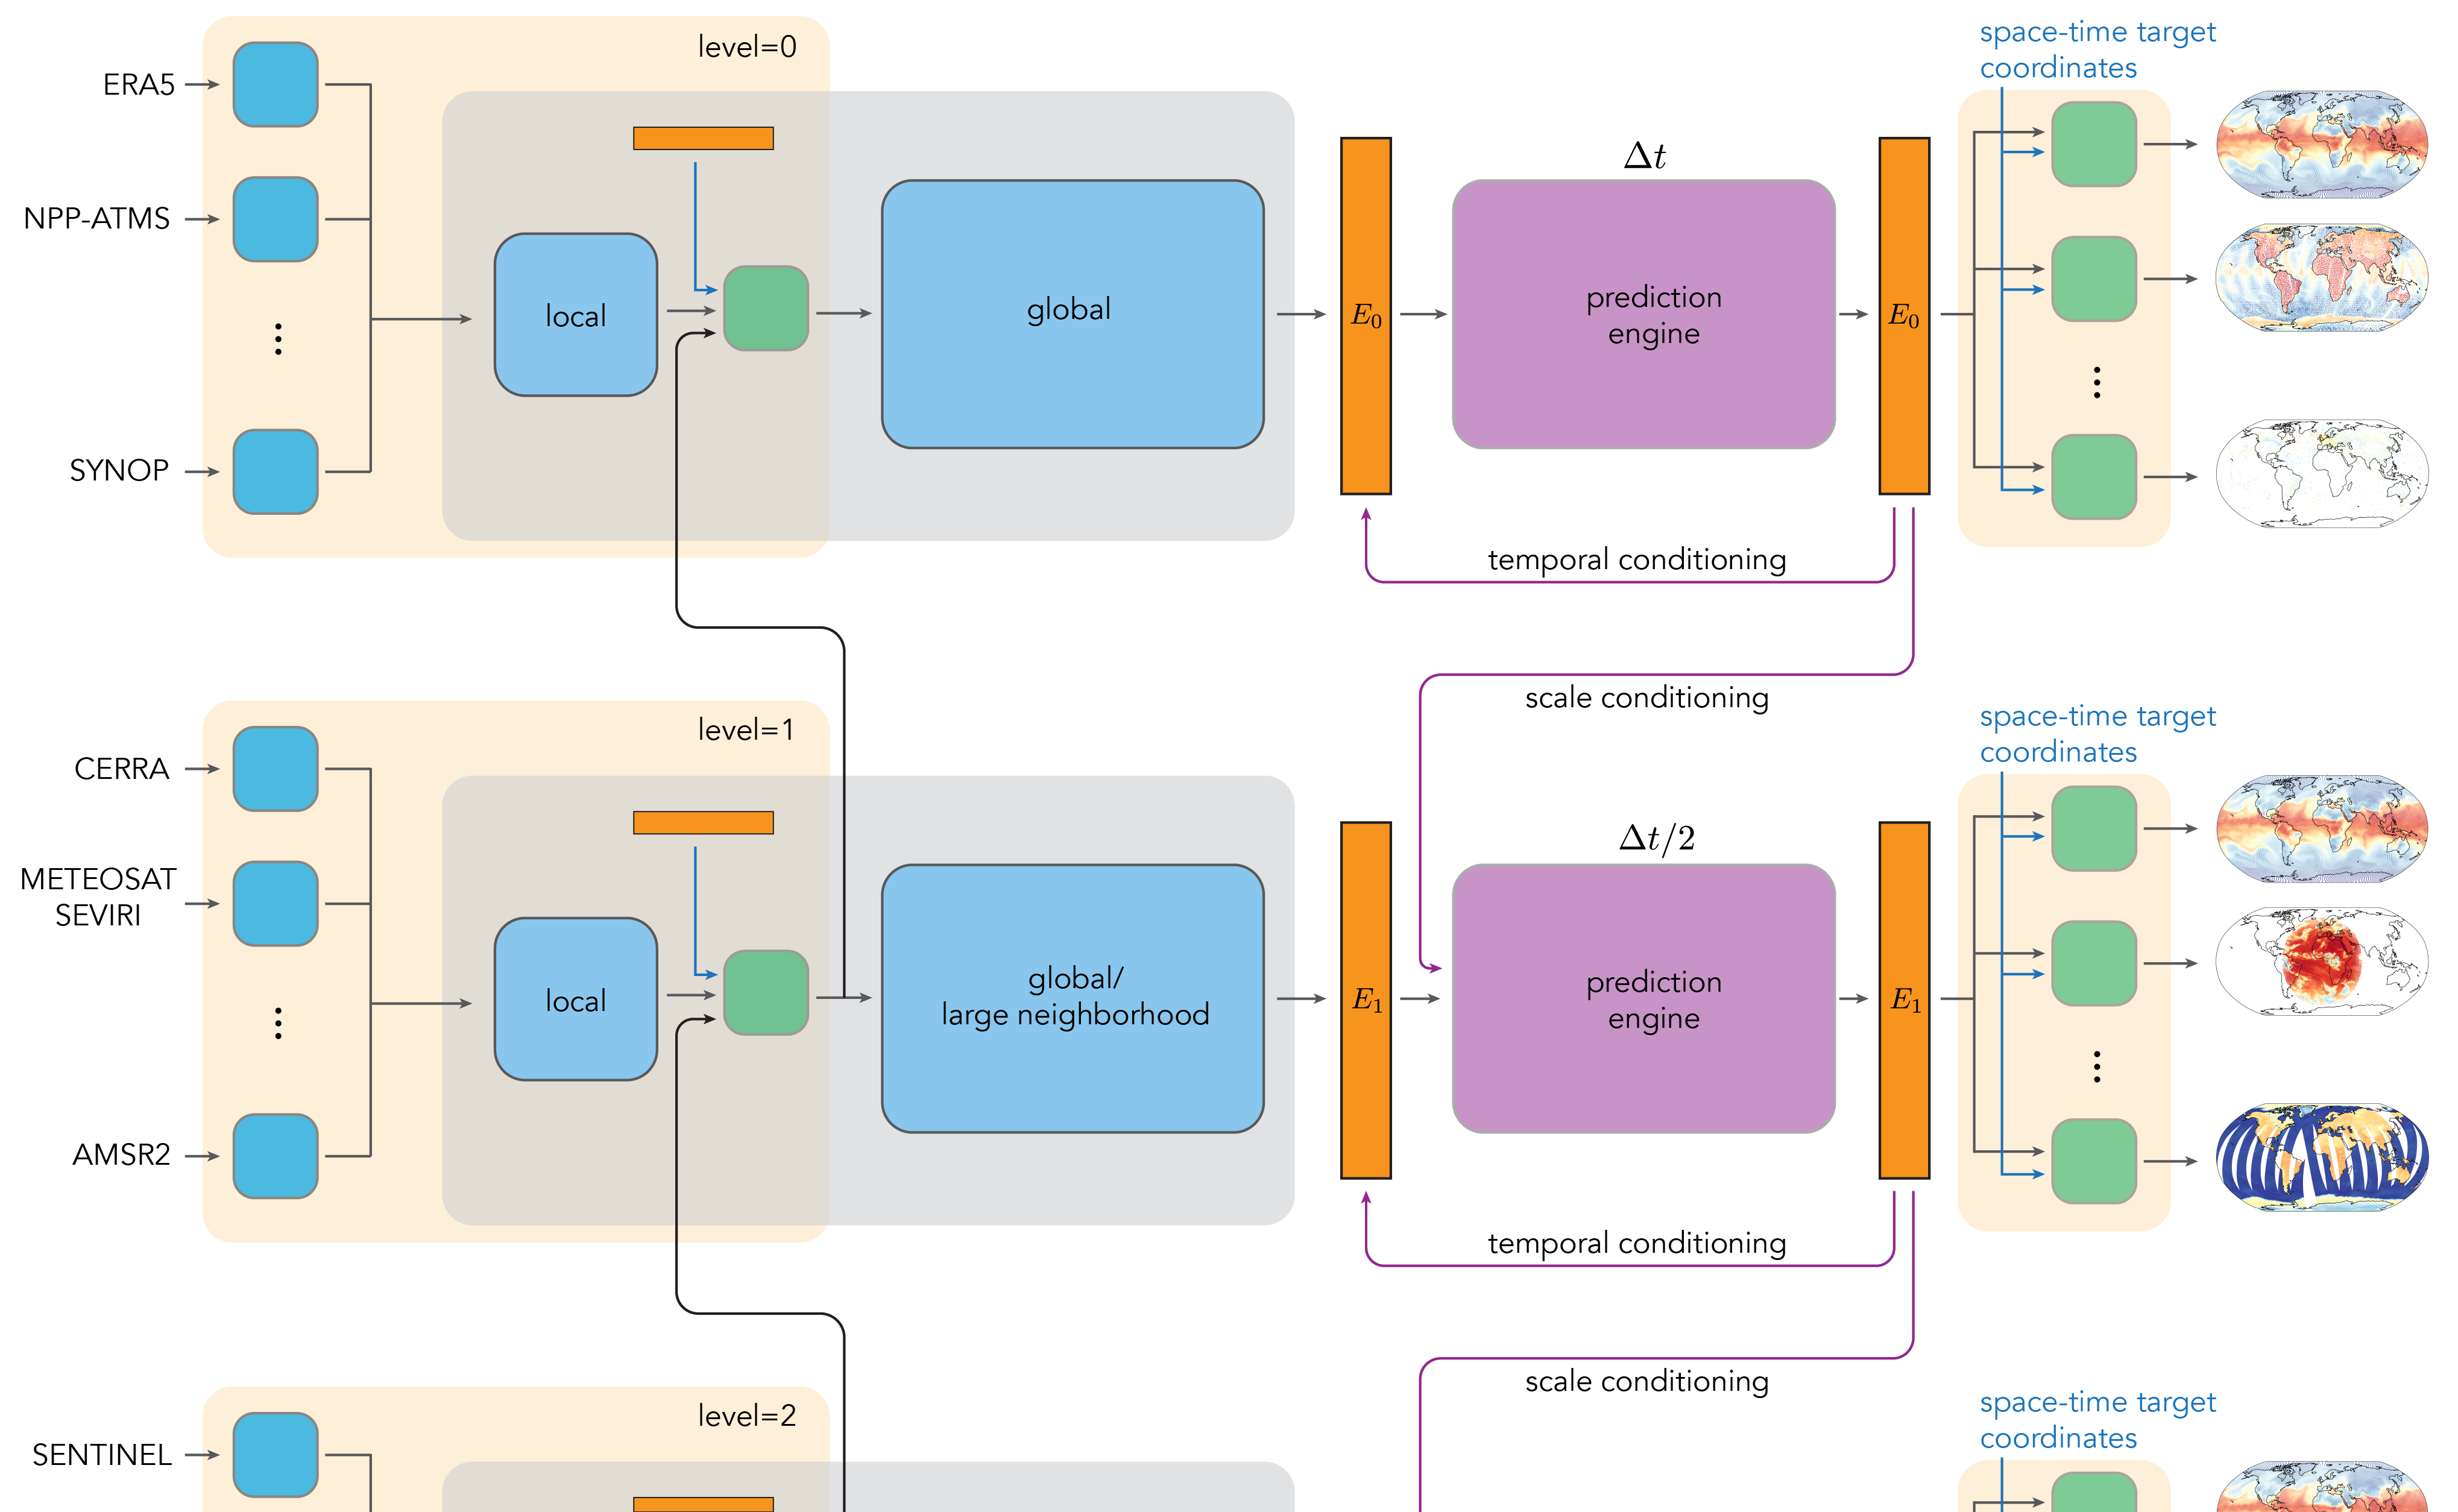
\includegraphics[width=0.9\textwidth]{figures/arch_mr.png}
    % 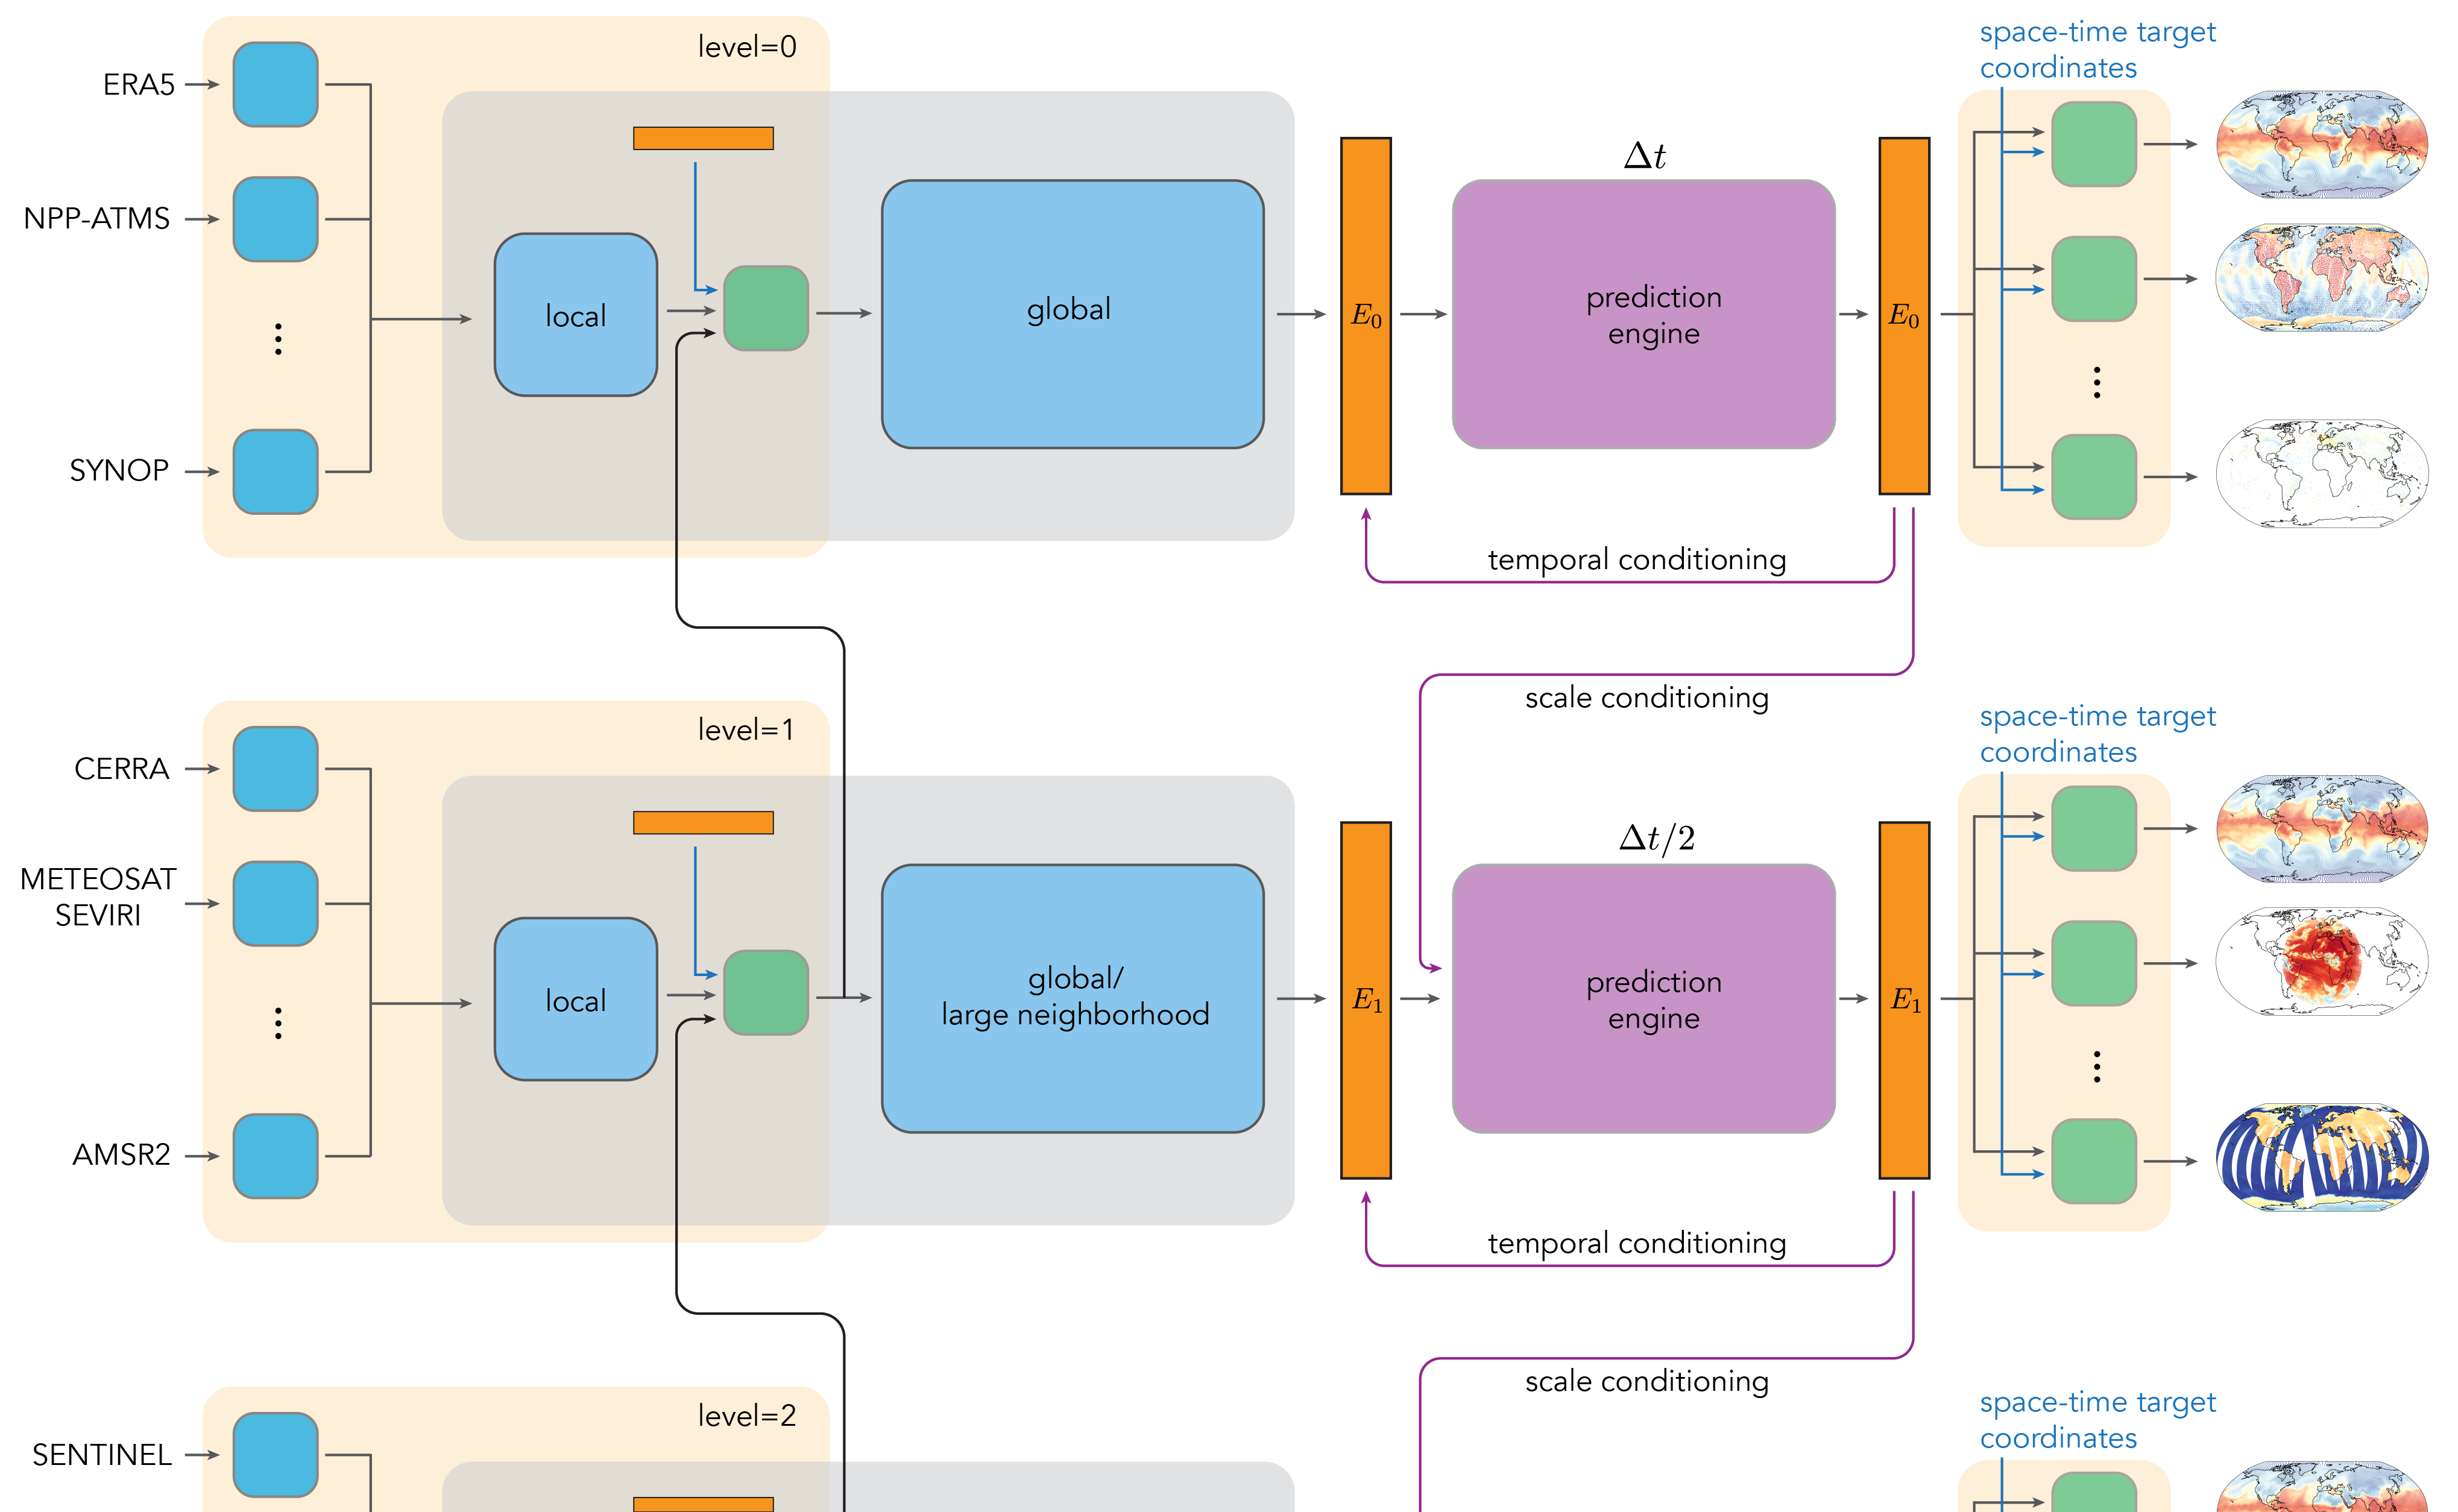
\includegraphics[width=0.9\textwidth]{figures/arch_mr.pdf}
    \caption{Envisioned multi-resolution structure for the WeatherGenerator. The column of conditional prediction networks is a multi-scale diffusion model similar to~\cite{Saharia2022}. From an Earth science perspective, it implements downscaling.  Forecasting with a conditioning on past information and a scale-adapted time step is also realized by the prediction engines $F_j$ that generate .}
    \label{fig:arch_mr}
\end{figure}

An important aspect of the WeatherGenerator is the ability to map between different representations.
For this, currently transformer read-out heads are employed.
These are cross attention heads that map a sequence of input tokens onto a set of read-out tokens; the approach was popularized by the Perceiver-IO architecture~\cite{Jaegle2021_Perceiver} although it is essentially nothing else than the cross-attention in the original transformer decoder~\cite{Vaswani2017}. %, see Fig XXX.
In particular, read-out heads are used to map from per dataset specific tokens to the global latent space and to provide predictions in physical space from the latent space.

More specificially, let $( X_i )_{i=1}^N$ be the set of input tokens and $( k_i^h )_{i=1}^N$ and $( v_i^h )_{i=1}^N$ be their projection onto the $h^{\textrm{th}}$ attention head.
Similarly, let $( q_i^h )_{i=1}^M$ be a set of head-specific query tokens, with $q_i$ being either learned or fixed but notably not dependent on the model input. 
The output tokens $\bar{q}_j^h$ are then defined by cross attention, i.e.
\begin{align}
  \bar{q}_j^h = \sum_{i=1}^N \sigma \big( q_j^h \cdot k_i^h \big) \, v_i^h 
\end{align}
where $\sigma$ is the softmax function.
The output of the multi-head attention module is, as usual, the concatentation of the per-head outputs $\bar{q}_j^h$ with a subsequent linear layer $L$ applied to it, i.e.
\begin{align}
  \bar{X}_j = L \big( \mathrm{cat}\big( \bar{q}_j^1 , \cdots , \bar{q}_j^H \big) \big) .
\end{align}

%%%%%%%%%%%%%%%%%%%%%%%%%%%%%%%%%%%%%%%%%%%%%%%%%%%%%%%%%%%%%%%%%%%%%%%%%%%%%%
\section{Next steps}
\label{sec:next_steps}

Two crucial aspects are missing in the current structure of the WeatherGenerator. 
One is a multi-scale structure in the in- and output. 
The second is to implement a multi-scale conditional latent diffusion model as the forecasting engine.
See Fig.~\ref{fig:arch_mr} for an overview.

%%%%%%%%%%%%%%%%%%%%%%%%%%%%%%%%%%%%%%%%%%%%%%%%%%%%%%%%%%%%%%%%%%%%%%%%%%%%%%
\section{The dirty details}

This section collects a more detailed view of the model architecture and the data flow through it. 

The input to the dataloader from the dataset classes is currently 
\section{Details on data flow in the code}
Here we will follow the flow of the ERA5 data through the network, specifying the dimensions of the tensors as a proxy for the functions and information flow. We are discussing the single input dataset case here.

Have a look at the forward function in the model class at this point. Also have a look at the diagram here in Fig~\ref{fig:dataflow}, which gives an idea of what goes into which function etc...

\begin{figure}[h!]
	\centering
	% 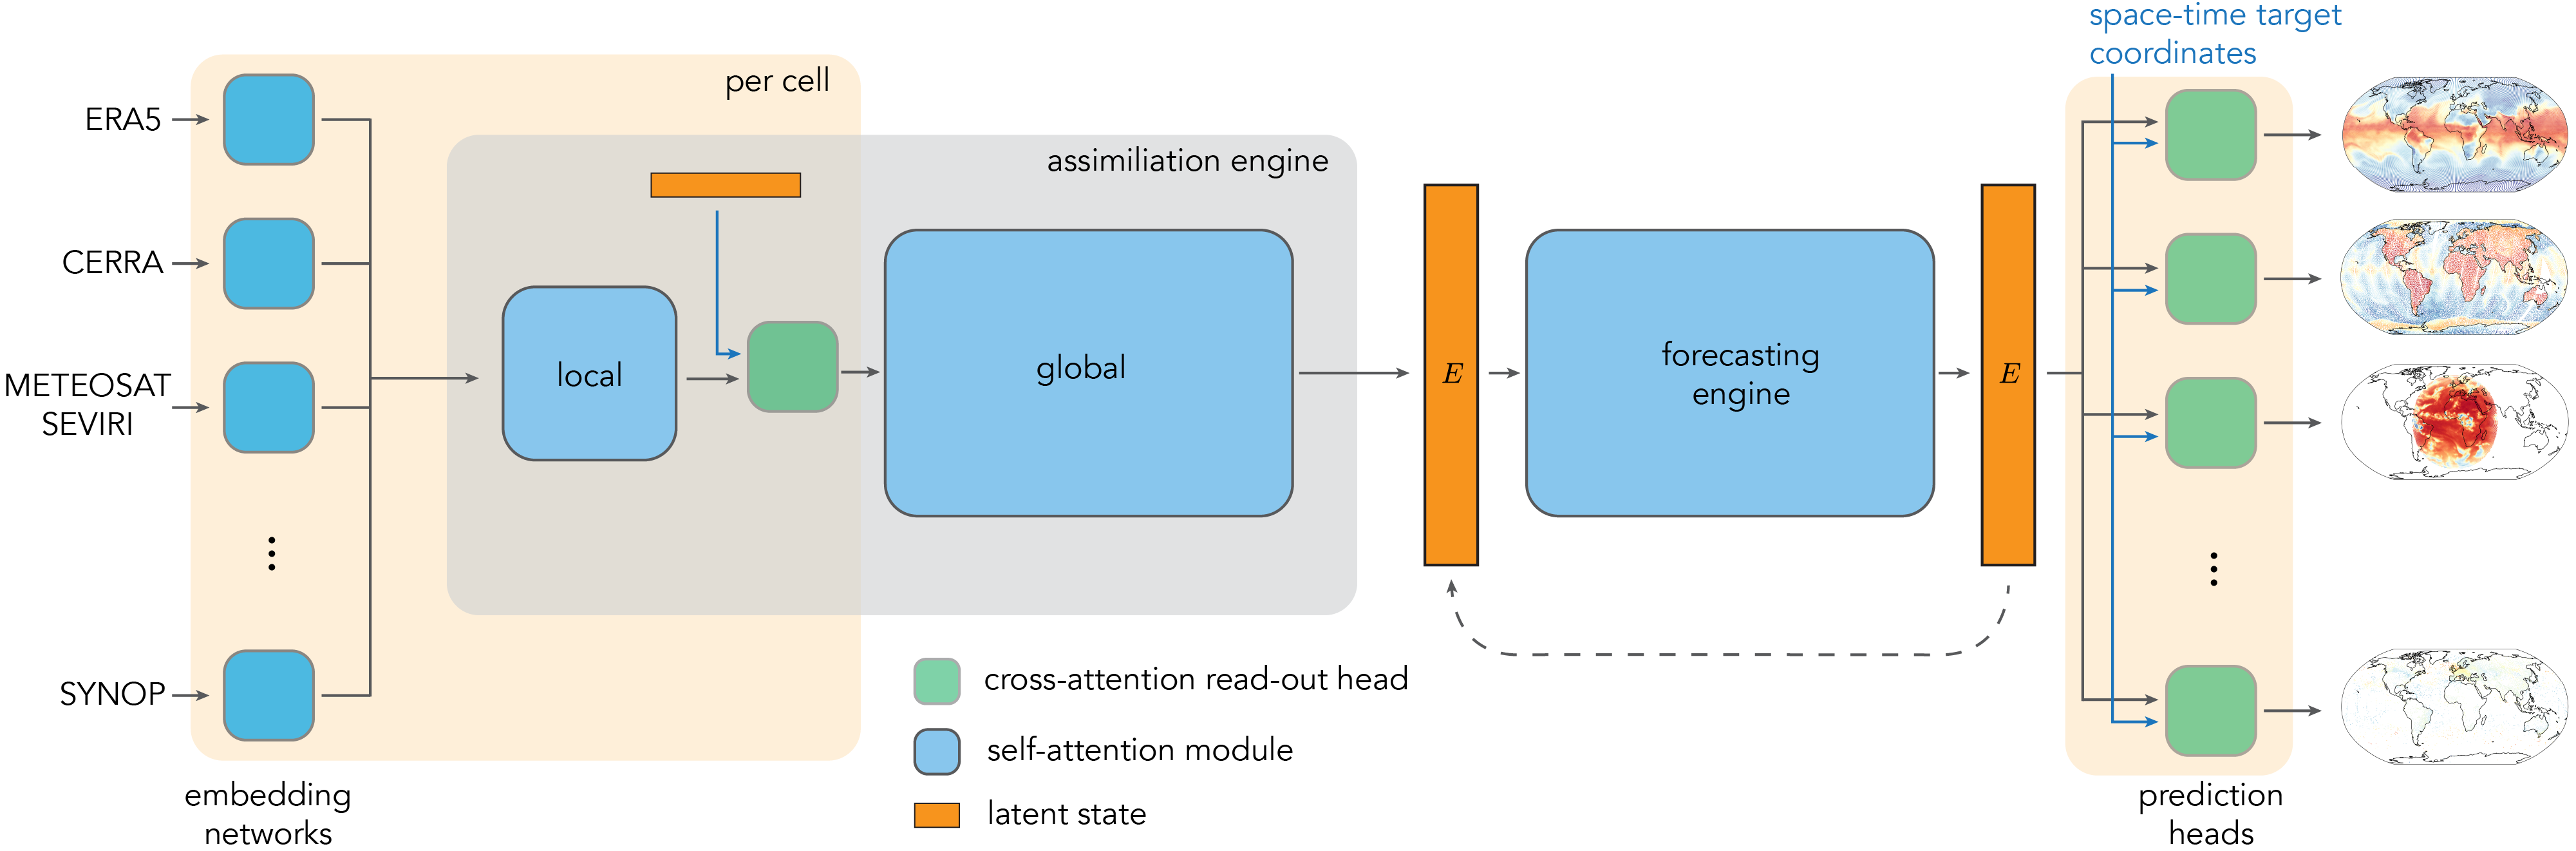
\includegraphics[width=\textwidth]{figures/arch.png}
    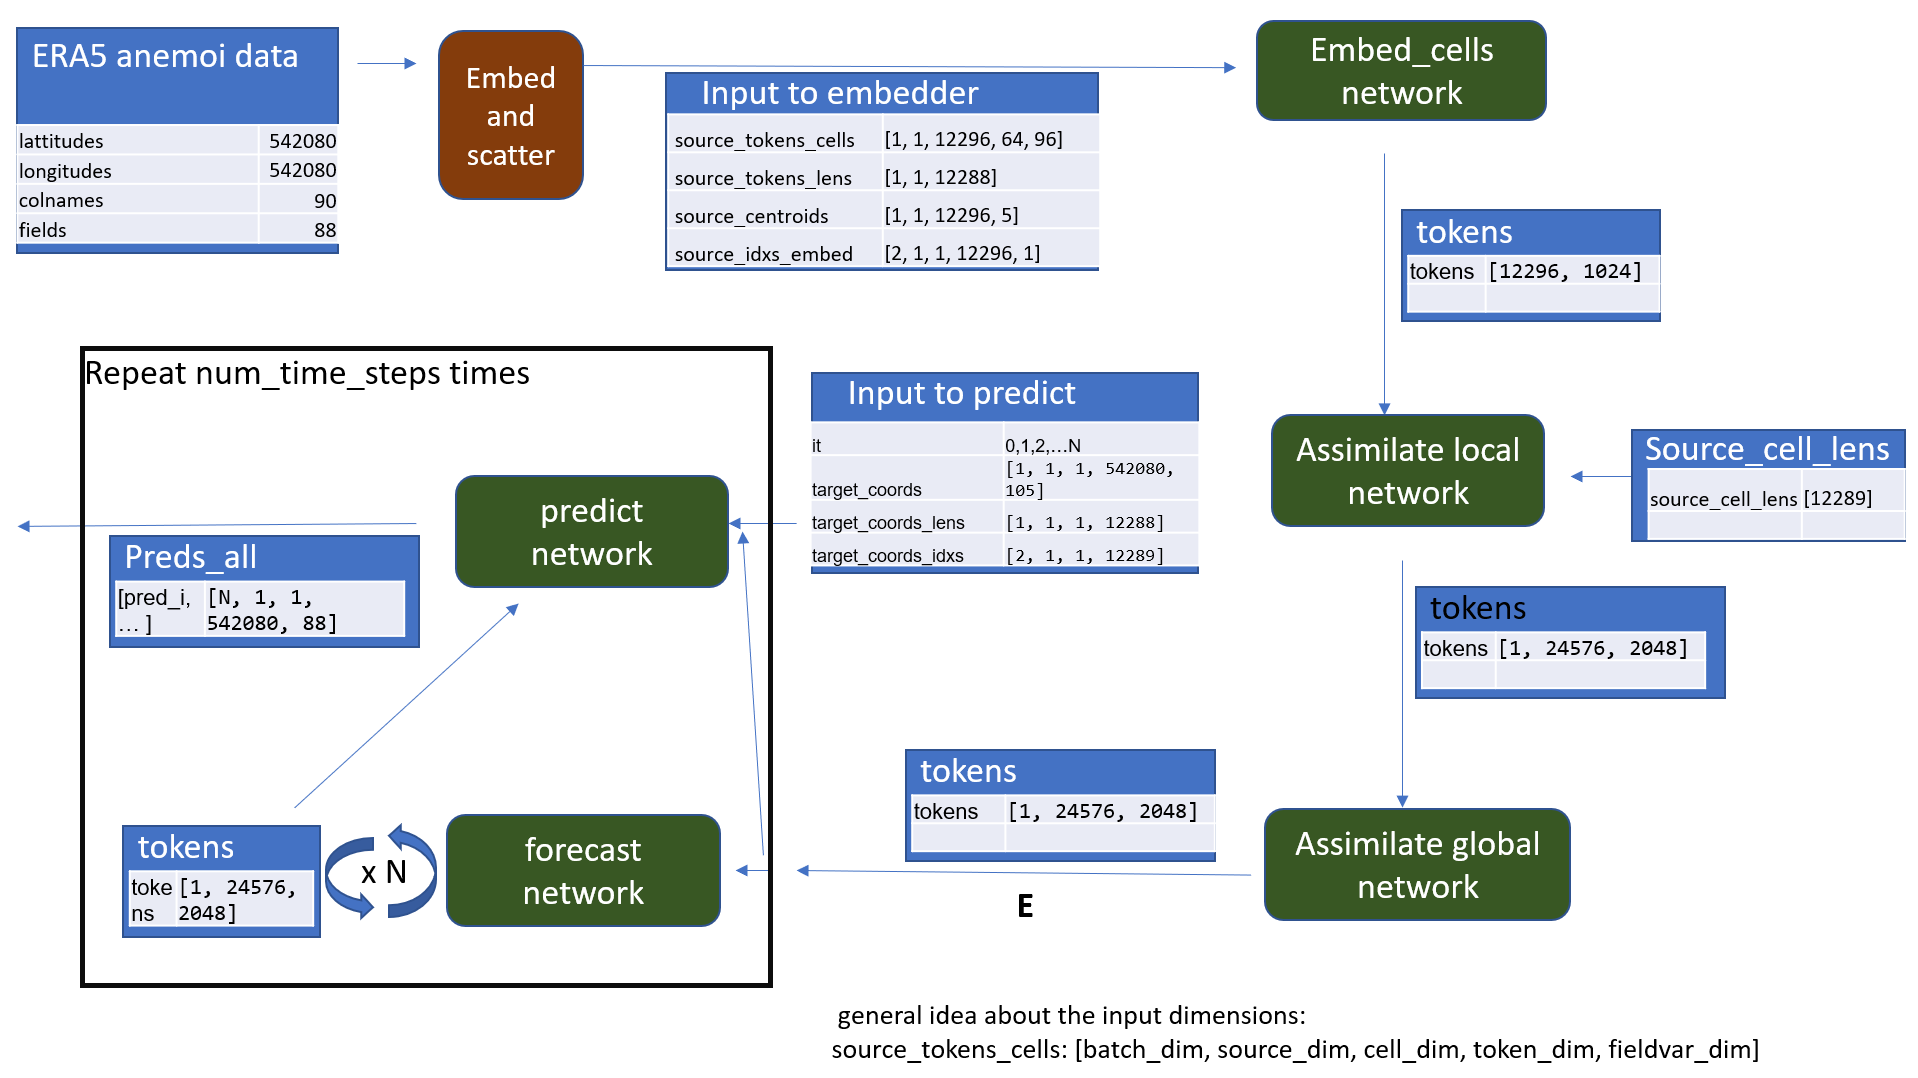
\includegraphics[width=\textwidth]{figures/dataflow.png}
	\caption{Diagram showing how data is flowing through the network}
	\label{fig:dataflow}
\end{figure}

% \begin{minted}{python}
% def forward( self, model_params, source_tokens_cells, source_tokens_lens, source_centroids,
%     source_cell_lens, source_idxs_embed, target_coords, target_coords_lens, target_coords_idxs,
%     num_time_steps) :

%     # some other steps
%     #...

%     # embed
%     tokens = self.embed_cells( model_params, source_tokens_cells, source_tokens_lens, 
%                                         source_centroids, source_idxs_embed)

%     # local assimilation engine and adapter
%     tokens = self.assimilate_local( model_params, tokens, source_cell_lens)

%     tokens = self.assimilate_global( model_params, tokens)

%     # roll-out in latent space
%     preds_all = []
%     for it in range( num_time_steps ) :

%       # prediction
%       preds_all += [ self.predict( model_params, it, tokens, 
%                                    target_coords, target_coords_lens, target_coords_idxs) ]

%       tokens = self.forecast( model_params, tokens)

%     # prediction for final step
%     preds_all += [ self.predict( model_params, num_time_steps, tokens, 
%                                   target_coords, target_coords_lens, target_coords_idxs) ]

%     return preds_all
% \end{minted}

\subsection{Input to the network}
The ERA5 data has around 0.4° resolution in lattitudes and 0.28° resolution in the longitudes, resulting in a total 542080 points on the lat/lon grid. Each of these 88 fields (temp, humiditiy etc) + 2 lat/lon coordinates, resulting in 90 columns in the zarr file.

\subsection{Initial Embed and scatter network ( self.embed\_cells( model\_params, source\_tokens\_cells, source\_tokens\_lens, source\_centroids, source\_idxs\_embed))}

First layer in the model is the embed cells, which consisty of two main functionalities:
\begin{enumerate}
    \item an embedding layer
    \begin{enumerate}
        \item this can be a transofrmer or a linear layer or something else
    \end{enumerate}
    \item and the scatter function
and the scatter function
\end{enumerate}

\subsubsection{Input dimensions}
The general dimenionality is like this: source\_tokens\_cells: [batch\_dim, source\_dim, cell\_dim, token\_dim, fieldvar\_dim], example: [1, 1, 12296, 64, 96].

The cell\_dim is in the simplest form how many healpix cells (areas) there are. For example for healpix\_level=5, there are 12288 cells. token\_dim is set as a parameter, that gives the maximum number of tokens per cell. So, let't say, if in a healpix cell, there are measurements on only 20 ERA5 grid points, then these twenty are simply appended by 44 0s to complete to the token\_dim parameter of 64. If, on the other hand, there are more ERA5 grid points in the cell, say in total 76 measurement points, then a new cell is created to catch the "spillage". These first 64 of the measurements fill the first cell, the rest 12 spill over to the new created cell and get appended by 52 0's to fill to 64. The variable source\_idxs\_embed keeps track of the spillage.

So we can say we have 12296 buckets that hold a max of 64 tokens inside, for each cell, when a bucket is not full, it gets filled with 0s; when it's full, we put the spillage into a new bucket. So we can have more buckets than cells.

\textbf{Remark:} Analysis shows that for bucket size of 64 and ERA5 data, we have 41 tokens per healpix cell in average. So in average in each bucket 41 are coming from ERA5, 23 are filled with zeroes. If we chose a bucket size of 16, then in average we would have 3 buckets per cell, since ceil(41/16) = 3.

\textbf{Note:} Kerem proposes to use the word bucket instead of cell after the tokens are distributed to the healpix cells, because after this, we have multiple buckets ("cells") that are associated with the same healpix cell etc, so for me calling both "cell" is confusing for me.

\subsubsection{Code}
The first loop for ib, sb in enumerate(source\_tokens\_cells) is over the batch dimension. The second loop for itype, (s,embed) in enumerate( zip(sb,self.embeds)) is over the source dimension.

Each source goes through the embedding network given in self.embeds, these are different for each source. The embedding is done per cell.

Then the function tokens\_all.scatter\_( 0, idxs, x\_embed + model\_params.pe\_embed[idxs\_pe]) puts all tokens together (from different batches and sources).

In the end, the tokens\_all have dimensions [12296, 1024], with 1024 the hidden\_dim. If we had two data streams (era5: source\_tokens\_cells[0][0] $=>$ [12296, 64, 96] and cosmo2: source\_tokens\_cells[0][0] $=>$ [3572, 64, 96]), then tokens\_all would be [15868, 1024].

So the output has the shape [12296, 1024] for ERA5.

\subsection{Local assimilation engine (tokens = self.assimilate\_local( model\_params, tokens, source\_cell\_lens))}
\subsubsection{Inputs}
This is still processing the data per cell.

The inputs are the tokens from before ([12296, 1024]) and the source\_cell\_lens, which is of size ([12289]). It looks like this [0, 1, 1, 1, 2, 1, 120, 1, ..., 8, 1, 1, ...], with most entries 1 and some $>$1. The first entry is set to 0 for technical purposes (making the length 12288+1=12289). Say the max entry in this vector is 131. This vector holds the information, how many token buckets (each with 64 tokens) there are in each cell. In the example here, we have the first three cells with one bucket each, then a cell with two buckets, then one cell with one bucket, then one cell with 120 buckets etc... We have one cell with 131 buckets.

As a sanity check: the sum of this vector source\_cell\_lens has to give us 12296. Or if we had two data sources (era5: source\_tokens\_cells[0][0] $=>$ [12296, 64, 96] and cosmo2: source\_tokens\_cells[0][0] $=>$ [3572, 64, 96]), then the sum of this vector would be 15868.

\subsubsection{The code}
The function implements a varlen attention mechanism. As we can have different number of tokens per cell (i.e. diff number of buckets) we need the varlen attention mechanism. It also uses the Perception IO idea to make the number of tokens independent of the number of input tokens. That is, the input may contain 2, 300, 25 or whatever many tokens per cell, the output will always be a fixed number of tokens. Concretely, in our example, we have 12288 cells. In our config we state how many tokens per cell we want (cf.local\_num\_queries), say local\_num\_queries=2, then we state we want 2 tokens per healpix cell regardless of how many tokens we have associated with that cell in the input. In this example we will end up with 12288*2=24576 tokens in total.

The fixed ouput number of tokens is implemented with the perceiver IO idea, that is the queries come from randomly initialized vectors instead of being formed from the input tokens. In the code the query vectors are given in q\_cells.

\textbf{Remark}: imagine we had set num\_tokens (bucket size) to 8 instead of 64. As stated before, with ERA5 we have in average 41 tokens per cell, that would mean we would have ceil(41/8)=6 buckets associated with each healpix cell in average. so i would have an input size similar to [73728, 1024] (73728=12288*6).  Then if i have local\_num\_queries=2, that is my output number of tokens is set to 12288*2=24576, that would lead to a token compression 73728 → 24576, that is a ratio of 73728/24576=3. So here one needs to be careful about this compression. Also be aware that this compression ration is not the same for all cells, as each cell has a different number of tokens/buckets...

Output: the code outputs the tokens in the size of [cf.local\_num\_queries*num\_healpix\_cells, 2048], in this example [24576, 2048]. 

\textbf{Question:} 2048 why is this 2048 and not 1024?

\subsection{Global assimilation engine (tokens = self.assimilate\_global( model\_params, tokens))}

\subsubsection{The Input}
This takes the tokens as inputs of size [24576,2048]. The idea here is to mix the information from the different healpix cells together for the first time. So it uses global as well as local attention blocks, the ratio is given by the parameter cf.ae\_global\_att\_dense\_rate, say if this is set to 0.2, then every 5th block is global attention.

%%%%%%%%%%%
%%%%%%%%%%%
\subsubsection{The Code}
The global attention layers use the full attention score matrix (24576x24576), although implemented with flex\_attn in the background without forming the full matrix.

The local attention matrices are implemented by providing a mask. The mask filters for neighboring healpix cells, taking only the closest n'th neighbors. Finding out which cells are neighbors is very easy in the healpix algorithm. In the healpix algorithm, if two cells belong to the same mother healpix cell, their indices have the same quotient when divided by 4. Simply, cells 1,2,3,4 belong to the same mother cell, 5,6,7,8 belong to another mother cell. 

Take, for instance cells number 154 and 149 in the Fig~\ref{fig:healpix} and say we want to find the mother cells two layers above. so we need to take floor division with $4^2=16$. floor(154/16)=9, floor(149/16)=9, so both of these belong to the same mother two levels above. If we want to go three levels above, we need floor division with $4^3=64$.

This masking is implemented in the code as where block factor=64 in our example. Have a look at the mask\_block\_local( batch, head, idx\_q, idx\_kv) function in the code at this point.
% \begin{minted}{python}
% def mask_block_local( batch, head, idx_q, idx_kv):
%       return ((idx_q // block_factor) // block_factor) == (idx_kv // block_factor)
% self.block_mask = create_block_mask( mask_block_local, B=None, H=None,
%                                          Q_LEN=qkv_len, KV_LEN=qkv_len)
% \end{minted}

An immediate idea here is to experiment with varying block factors for different heads, that is, different heads looking at neighbors at different healpix levels.
\begin{figure}[h!]
	\centering
	% 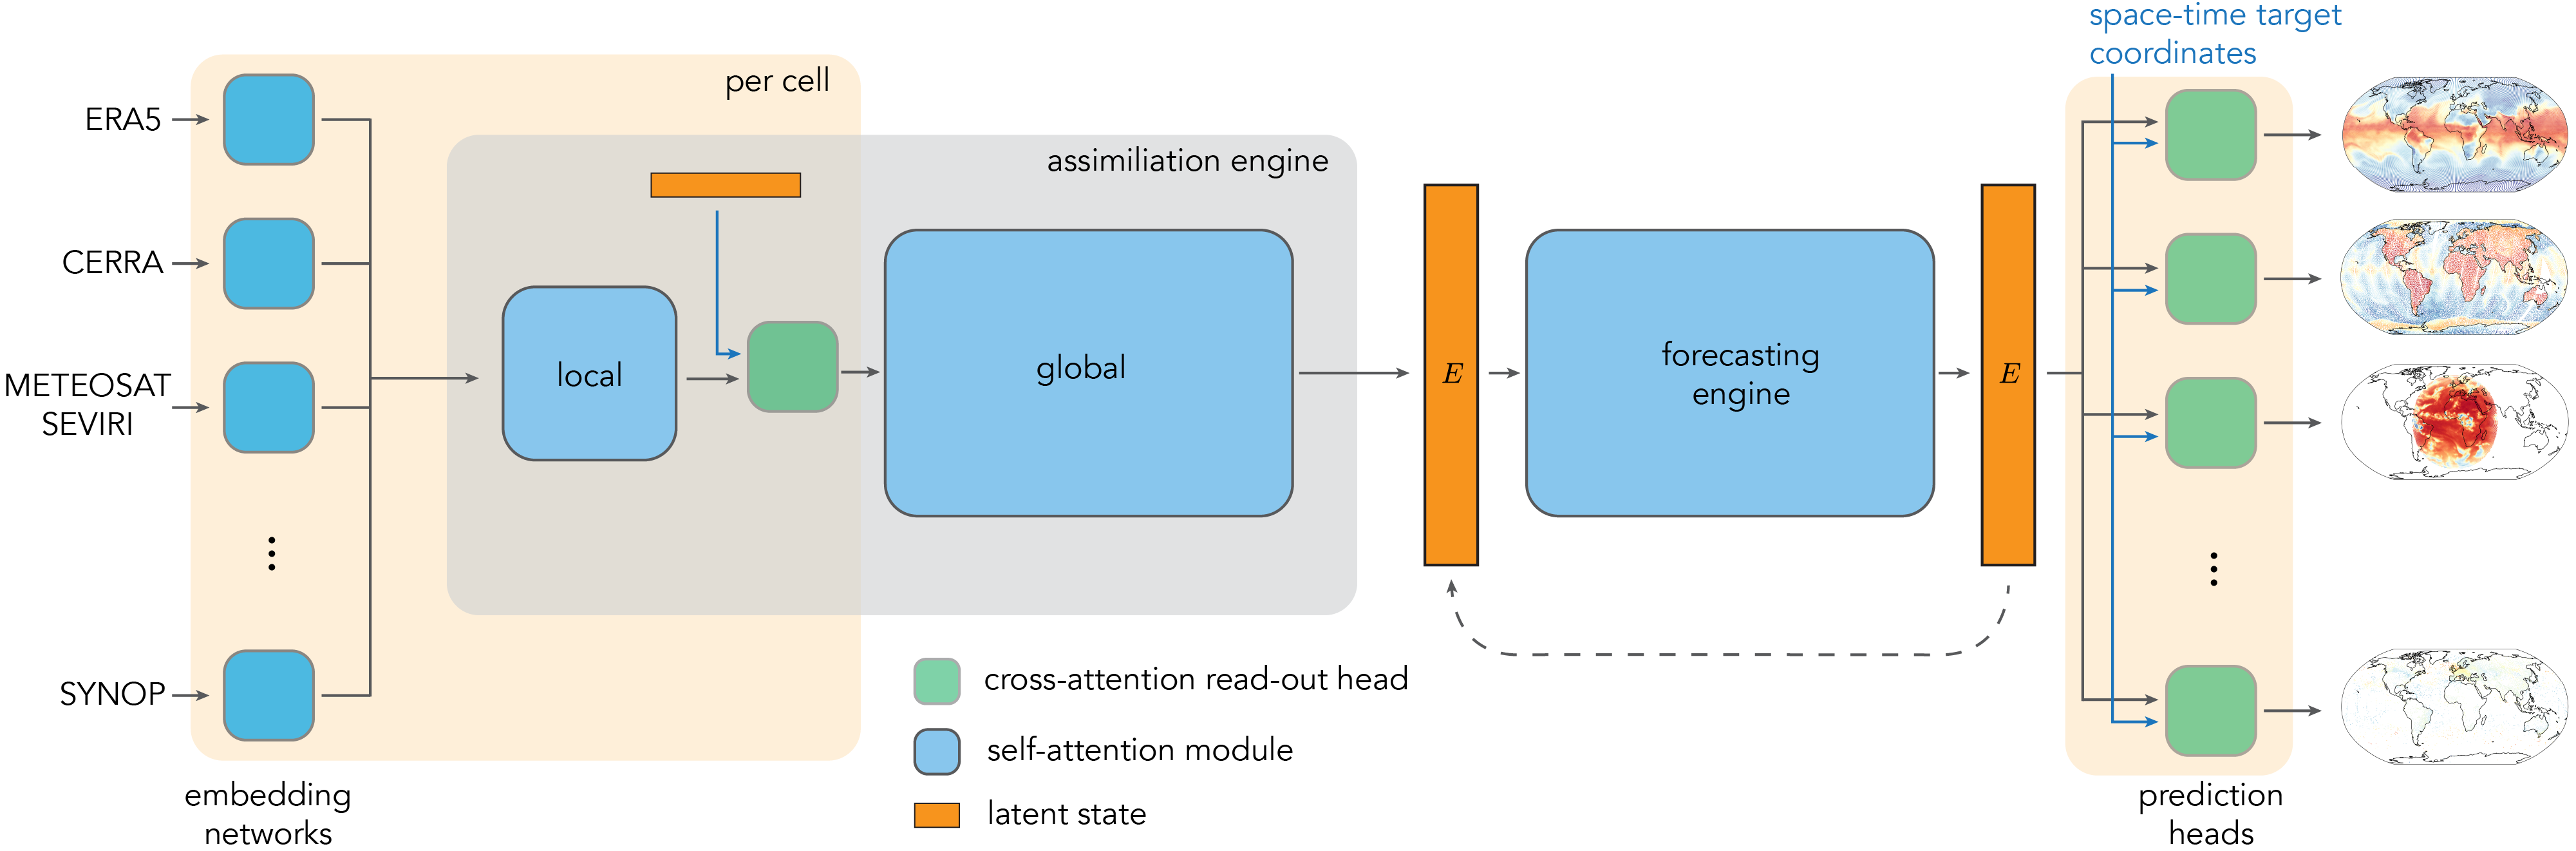
\includegraphics[width=\textwidth]{figures/arch.png}
    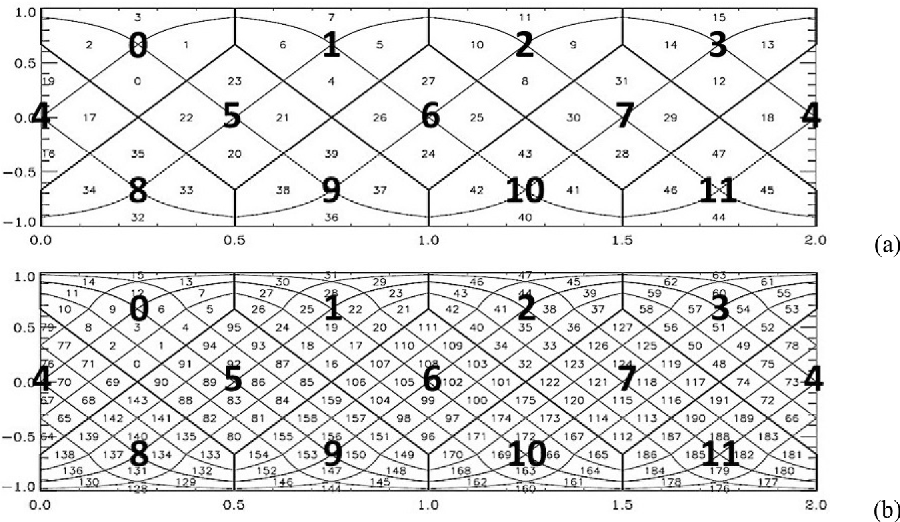
\includegraphics[width=\textwidth]{figures/healpix_demo.png}
	\caption{Healpix}
	\label{fig:healpix}
\end{figure}

\subsubsection{Output}
the global assimilation network mixes info together from the different cells and outputs tokens of size [1, 24576, 2048]. 

\subsection{Predict network (self.predict( model\_params, it, tokens, target\_coords, target\_coords\_lens, target\_coords\_idxs))}

this is called in a an iterative manner in the rollout loop, 0 to num\_time\_steps. this also uses varlen attention, implementing the perceiver IO to go from a fixed number of tokens to variable output sizes.


\subsubsection{Input}
Inputs are the tokens from the global engine and the prescribed output coordinates.

\begin{table}[]
\begin{tabular}{|l|l|l|}
\hline
target\_coords & [1, 1, 1, 542080, 105] & 542080: number of lat/lon grids, 105: coordinates in different coordinate systems \\ \hline
 target\_coords\_lens   & [1, 1, 1, 12288]     &  again tells us how many buckets per cell, sth like [41, 41, 42, ..., 41, 70, 41, ...]   \\ \hline
  target\_coords\_idxs  &   	[2, 1, 1, 12289]   &    \textbf{Question: what is the logic here?} \\ \hline
\end{tabular}
\end{table}

\textbf{remark:} if we have two stream, era5 and cosmo2, then

 target\_coords[0][0][0]: Tensor shape=torch.Size([226980, 105])

target\_coords[0][0][1]: Tensor shape=torch.Size([542080, 105]),

similarly 

target\_coords\_lens[0][0][0]: Tensor shape=torch.Size([12288]), dtype=torch.int64, device=cpu
target\_coords\_lens[0][0][1]: Tensor shape=torch.Size([12288]), dtype=torch.int64, device=cpu


\subsection{Forecast network (tokens = self.forecast( model\_params, tokens))}
This takes the tokens as input, advances them and spits out the advanced tokens in the same format.


\appendix

\section{Multi-resolution architecture}

An overview of the envisioned multi-resolution structure is give in Fig.~\ref{fig:arch_mr}.

\begin{figure}[t]
	\centering
	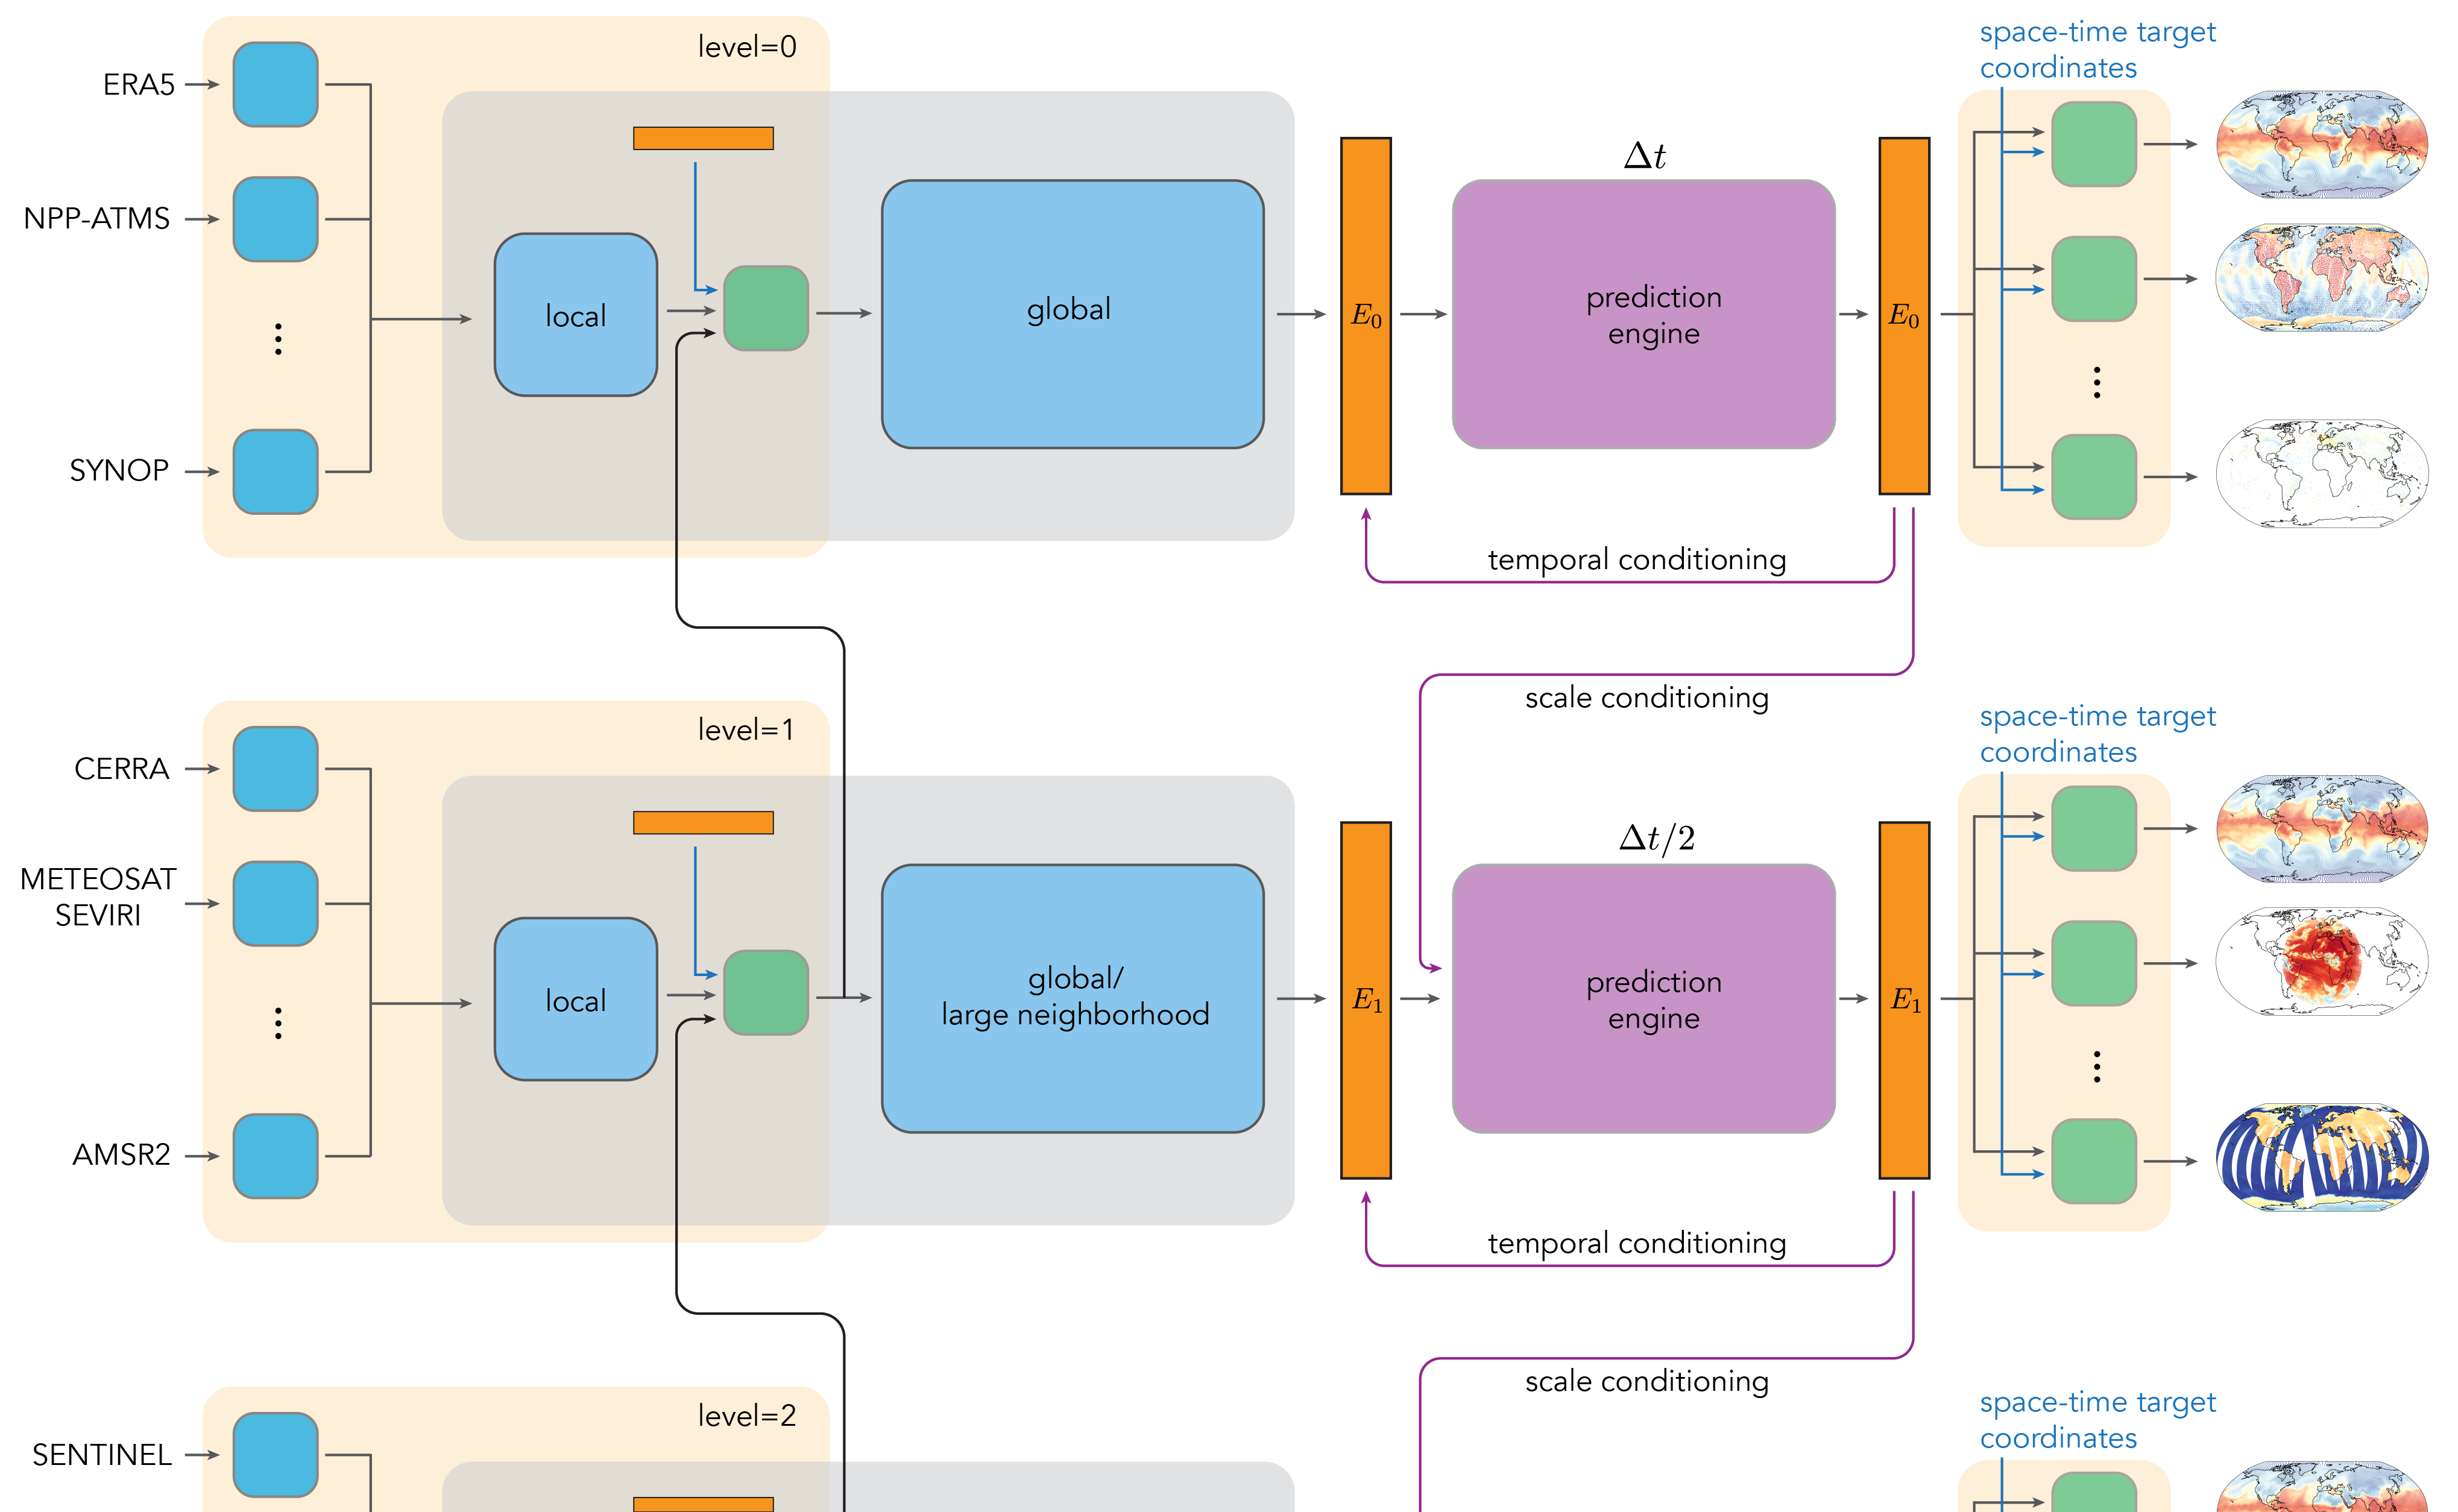
\includegraphics[width=\textwidth]{figures/arch_mr.png}
    % 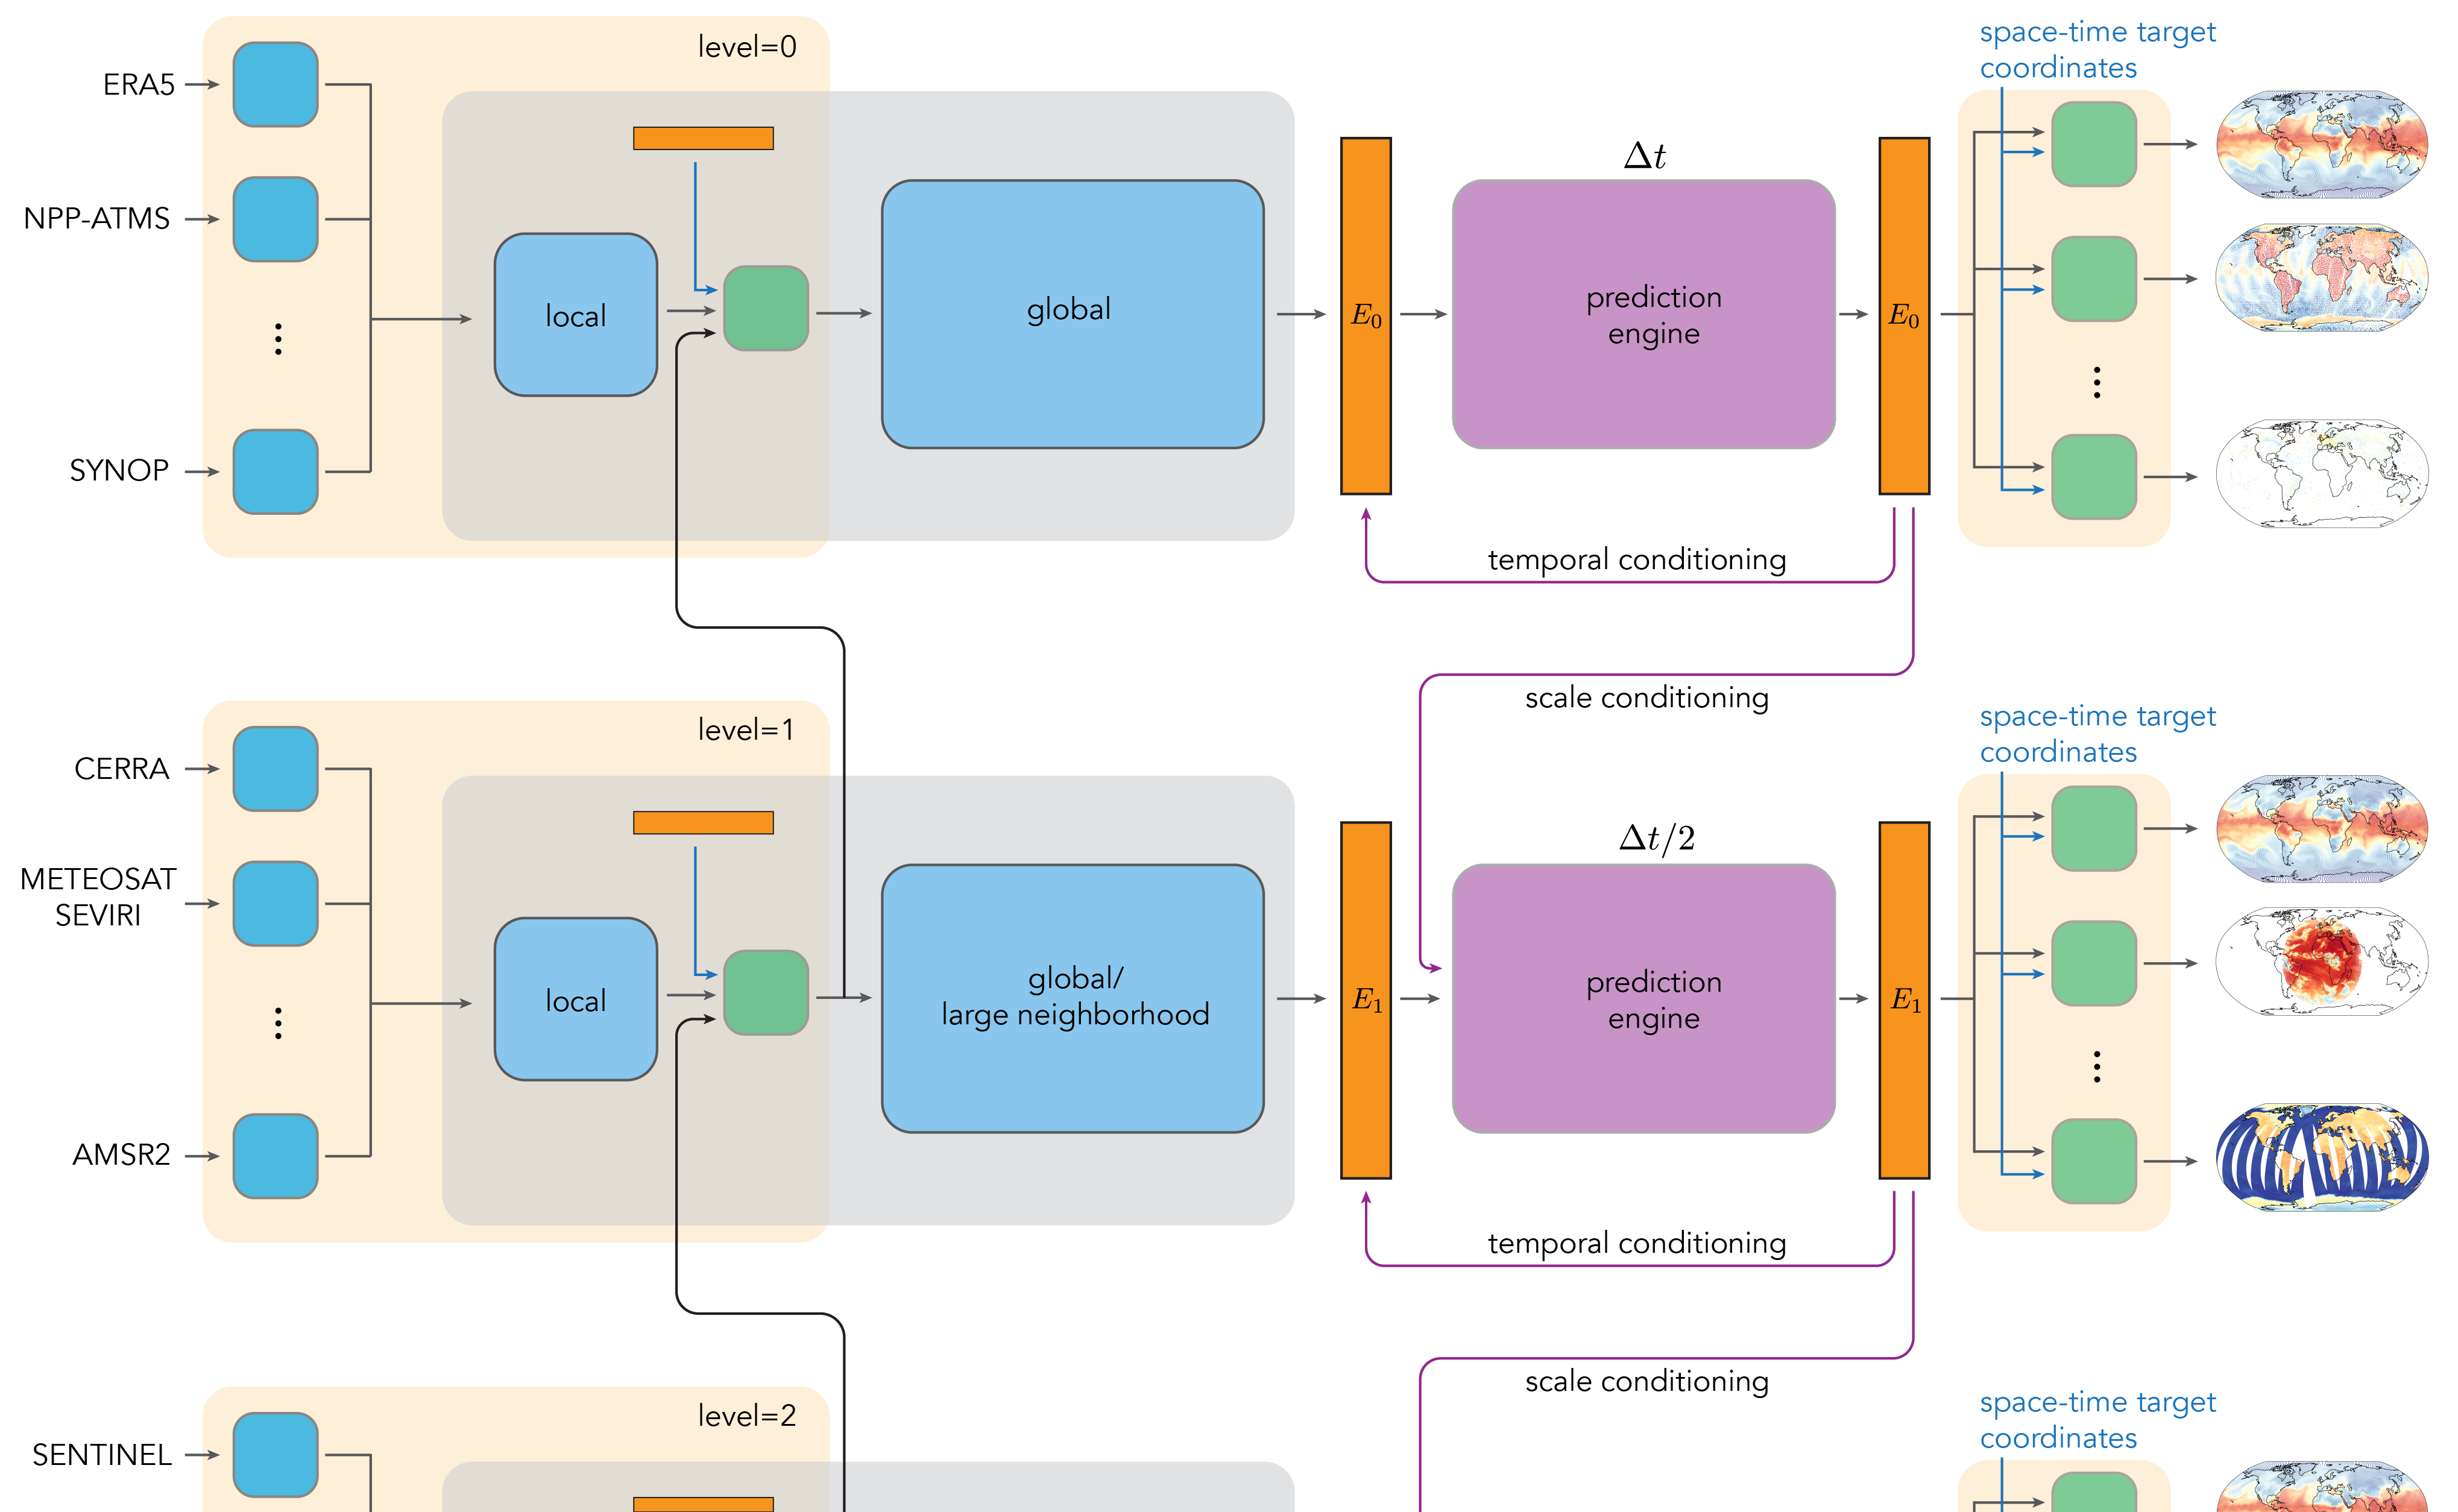
\includegraphics[width=\textwidth]{figures/arch_mr.pdf}
	\caption{Overview of the WeatherGenerator neural network architecture}
	\label{fig:arch_mr}
\end{figure}


\bibliographystyle{alpha}
\bibliography{references}

\end{document}
